%%%%%%%%%%%%%%%%%%%%%%%%%%%%%%%%%%%%%%%%%%%%%%
\logvartrue
\chapter{A life in transition: bacteria in harsh environments}
%%%%%%%%%%%%%%%%%%%%%%%%%%%%%%%%%%%%%%%%%%%%%%
Bacteria are everywhere and they make up for their small dimensions in sheer number. Thanks to their flexible metabolism, bacteria have been able to thrive in almost all environments on the heart, from acid mines to sulphur pools. However, studying bacterial communities in such environments can be very difficult since, as said, only a small fraction of bacteria can be isolated under standard laboratory conditions. Indeed, it is estimated that in a single gram of soil live more than 4000 different bacterial ``genomic units'' based on DNA - DNA re-association studies. To overcome these limitations imposed by existing laboratory techniques, many future efforts should be focused on the direct sequencing of environmental DNA in order to extract all genetic informations contained in an environment. For this reason we have focused our attention to the study of bacterial communities in harsh environments using a sequence-driven approach based on the 16S rRNA gene sequences. This approach has allow us to retrieve informations about microbial populations not otherwise obtainable with standard microbiology techniques.\\

\section{Composition of supralittoral sediments bacterial communities in a Mediterranean island}
\newpage
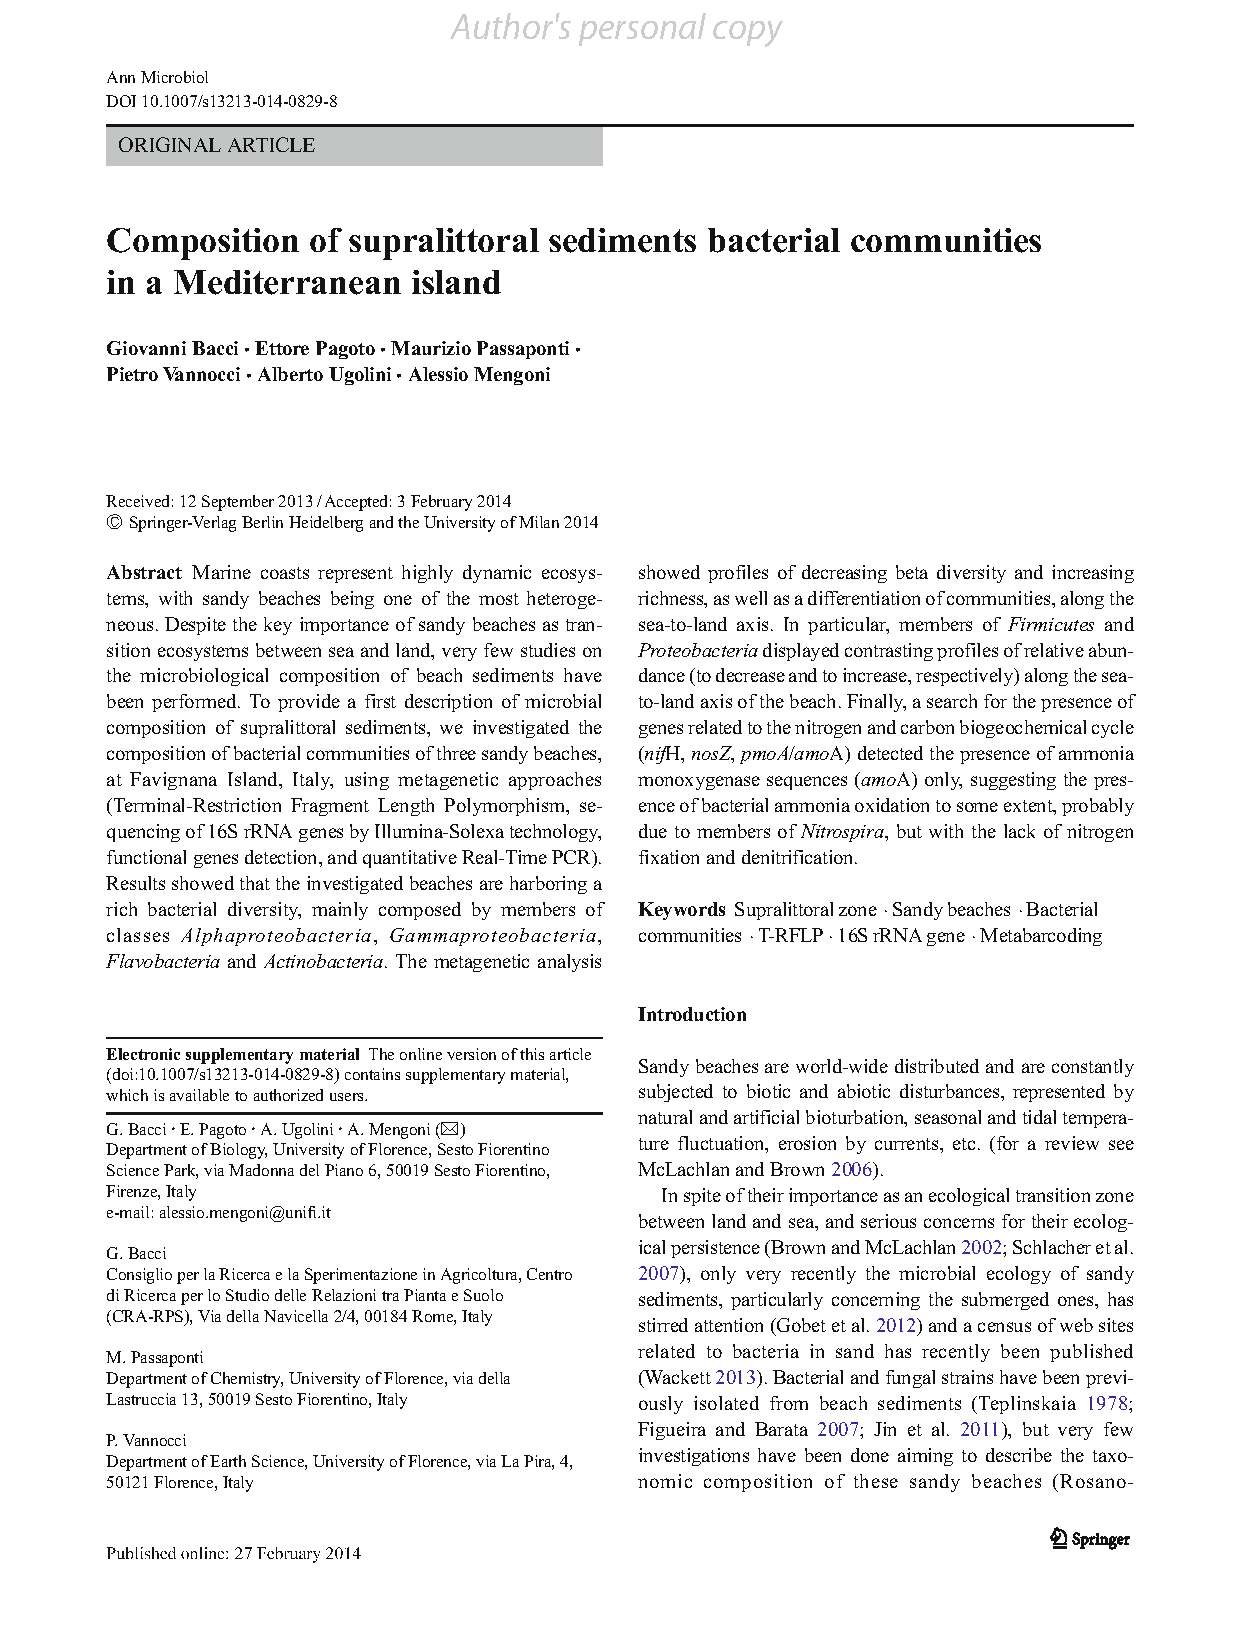
\includepdf[pages=-,offset=10mm 0, scale=0.9]{articles/favignana_mod.pdf}
\newpage

\section{Rhizosphere effect and salinity competing to shape microbial communities in Phragmites australis (Cav.) Trin. ex-Steud}
\newpage
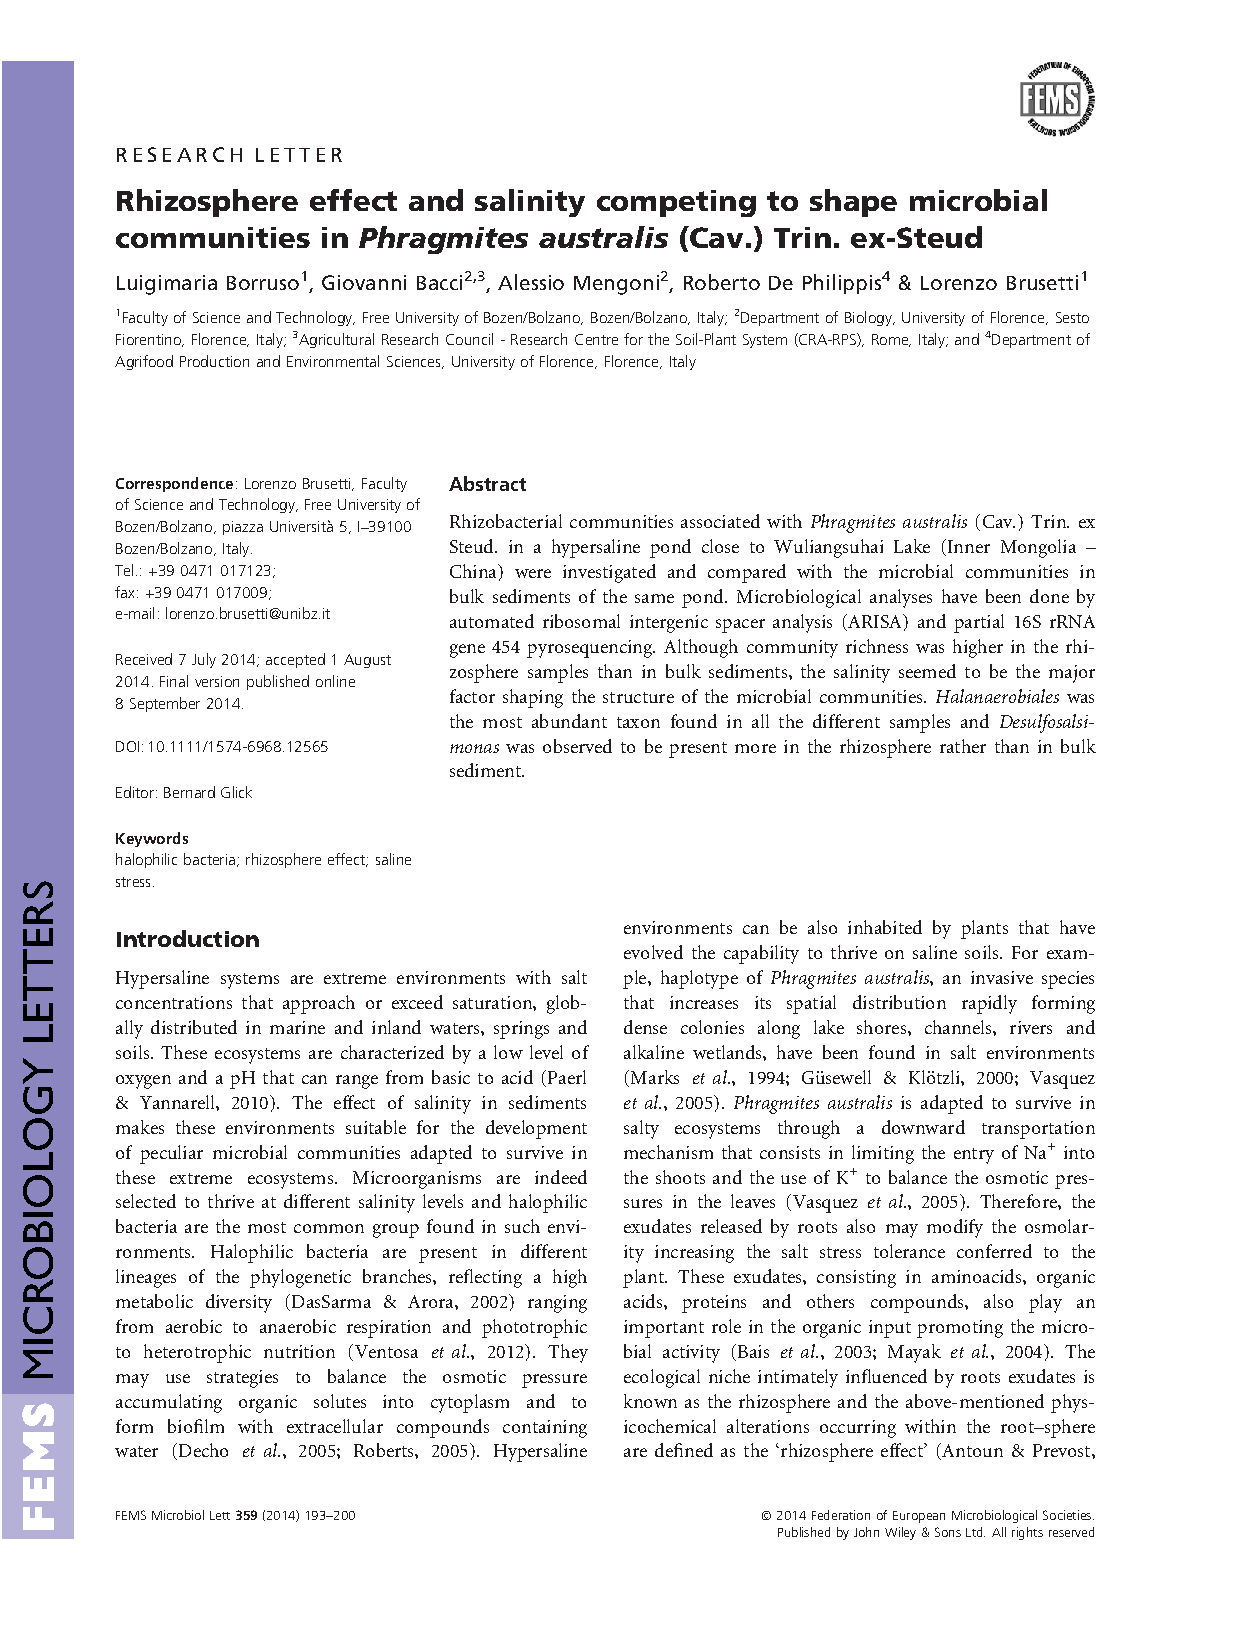
\includepdf[pages=-,offset=10mm 0, scale=0.9]{articles/borrusio.pdf}
\newpage

\section{Salinity and Bacterial Diversity: To What Extent Does the Concentration of Salt Affect the Bacterial Community in a Saline Soil?}
\newpage
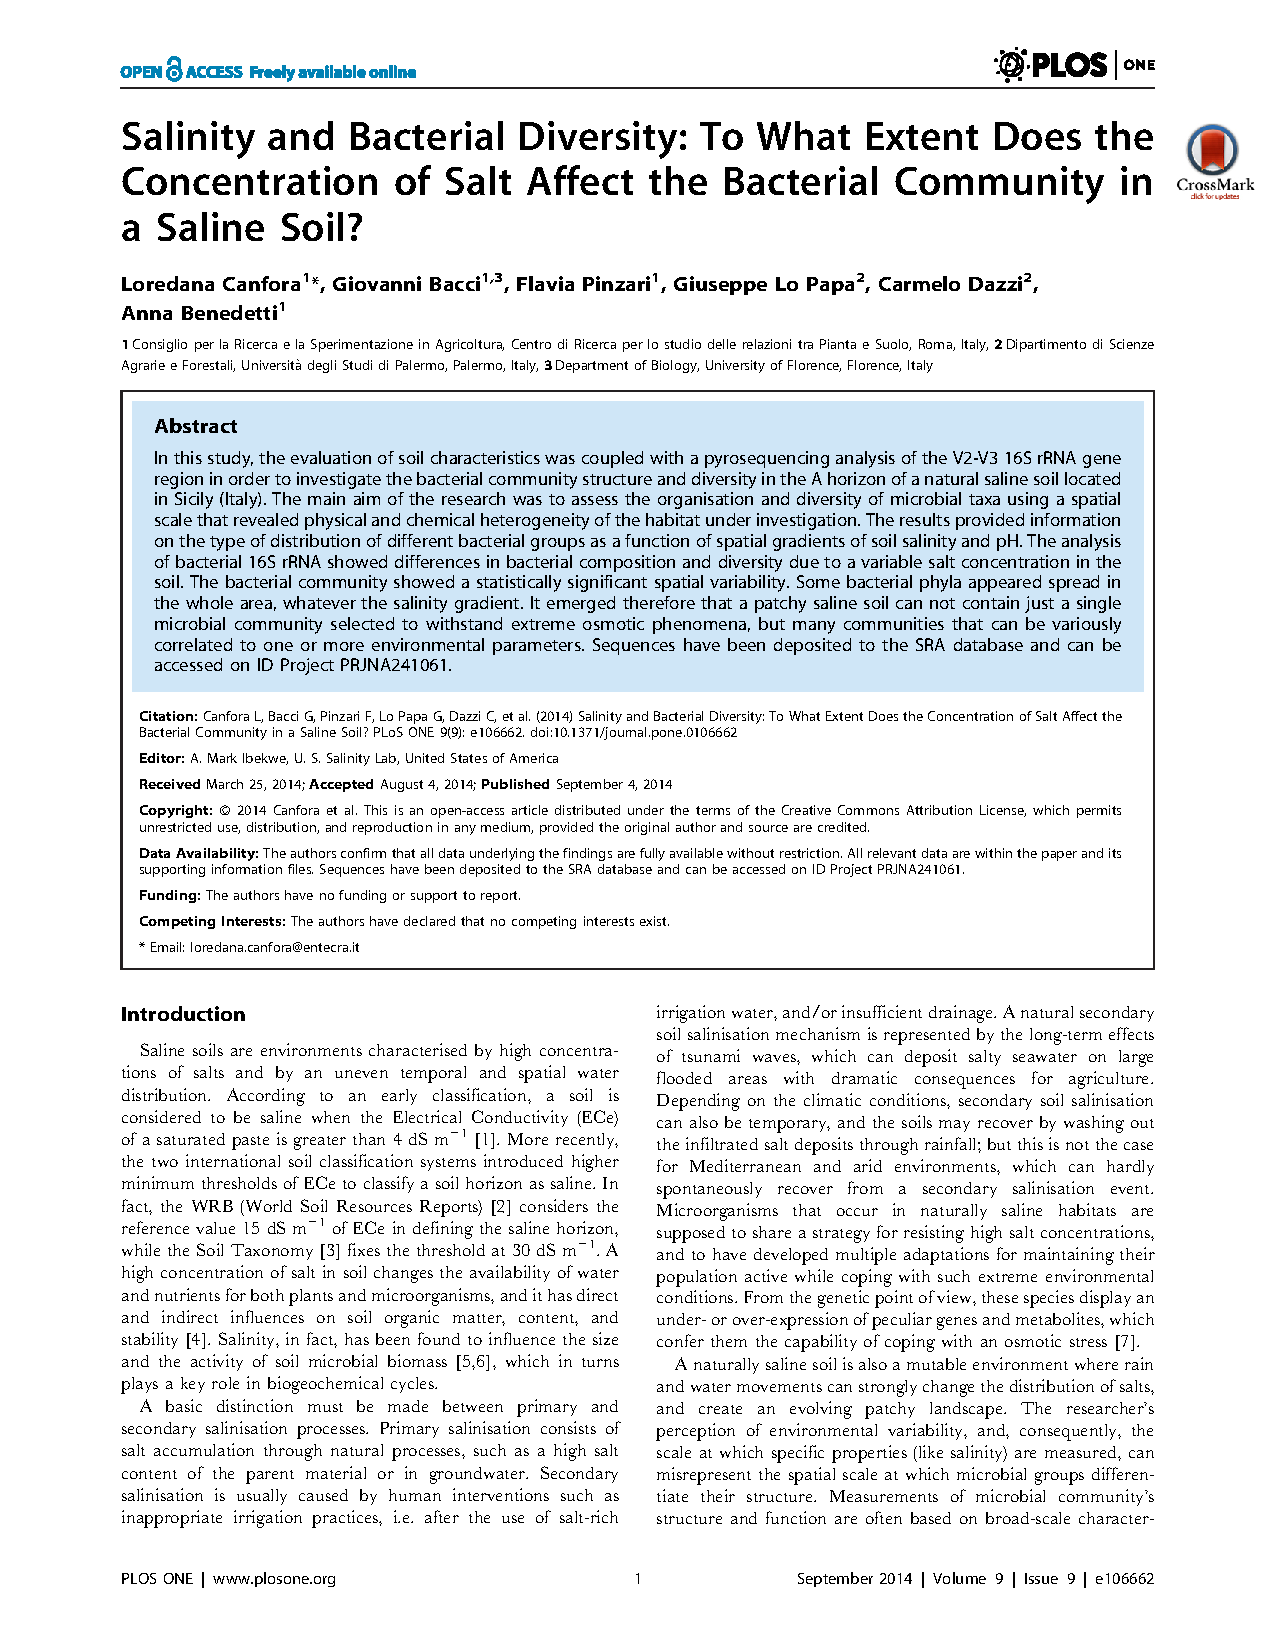
\includepdf[pages=-,offset=10mm 0, scale=0.9]{articles/loredana.pdf}
\newpage


%%-----------
%% Backmatter
%%-----------
\backmatter
\chaptermark{Bibliography}
\renewcommand{\sectionmark}[1]{\markright{#1}}
\bibliographystyle{unsrt}                           %Use alpha codes for references
\sectionmark{Bibliography}
\addcontentsline{toc}{chapter}{Bibliography}        %Force addition of Bibliography to TOC    
\bibliography{References}